Для работы модели нужно определить ее гиперпараметры. Рассмотрим две идеи: 

Первая идея (Train, validation and test stage, метод отложенной выборки): обучить модель по части train и по предсказаниям на второй части определить оптимальные гиперпараметры. Минус такого подхода в том, что модель будет зависить от случайного выбора части train (а вдруг объекты в train упорядочены по алфавиту и не все объекты попадут в обучающую выборку при определении гиперпараметров. Модель с этими гиперпараметрами может показать плохой результат на всей обучающей выборке).

Вторая идея (кросс-валидация): часть объектов идет на валидацию, часть на train, затем
данный процесс повторяется несколько раз (часть с валидацией меняется). Тогда мы можем измерить
дисперсию ошибки для каждого набора гиперпараметров и сам лосс, чтобы выбрать оптимальный набор гиперпараметров.

\textbf{Подробнее про Train, validation and test stage:}

\begin{figure}[h]
\centering
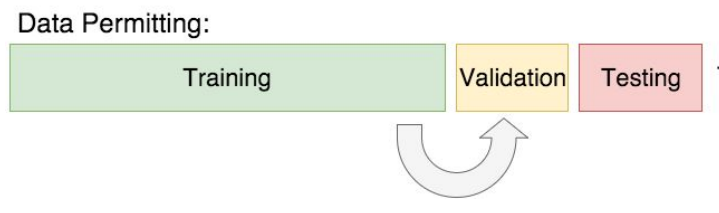
\includegraphics[width=0.5\linewidth]{13.4.PNG}
\caption{Train, validation and test.}
\end{figure}

\textit{Тренировочная выборка} - часть полной выборки, на котором мы обучаем модель. 

\textit{Валидационная выборка} - часть полной выборки, происходит настройка гиперпараметров. Это мы и назовём валидированием или валидацией модели. Изначально человек из каких-то знаний, опыта и других соображений выбирает некоторый пул гиперпараметров для текущей задачи. И далее по ним с каким-то шагом запускаем модель и проверяем получившиеся
предсказания с помощью метрик качества модели. Выбирает и фиксирует значения гиперпараметров.

\textit{Тестовая выборка} - часть полной выборки, который мы заранее отложили и проверяем значение функции потерь, а также метрики качества модели.
НЕ НАДО ВАЛИДИРОВАТЬСЯ НА ТЕСТОВОЙ ВЫБОРКЕ. Считайте, что проверка на тестовой выборке - это как финальная проверка работы. Уже с оптимизированными параметрами и гиперапараметрами запускаем модель, чтобы проверить её качество на этой части данных. Иногда для конечного теста, в тестовую выборку докидывают и валидационный датасет, но такой шаг является спорным.

\textbf{Overfitting problem, ways to detect it.}

\textbf{Определение.} Недообучение — ситуация, когда модель уловила не все общие закономерности и не способна достаточно точно воспроизвести распределение, из которого создаются объекты. Недообучение связано с тем, что по каким-то причинам алгоритм не уловил закономерностей в данных. Это явление, обратное переобучению, при котором алгоритм не полностью использует предоставленные ему для обучения данные.

\textbf{Определение.} Переобучение — ситуация, когда модель не только успешно смоделировала распределение, но и включила в него шумовые факторы (то есть переобучилась под выбросы). То есть построенная модель хорошо работает на объектах из тестовой выборки, но плохо работает на объектах, не участвовавших в тестовой выборке.

\begin{figure}[h]
\centering
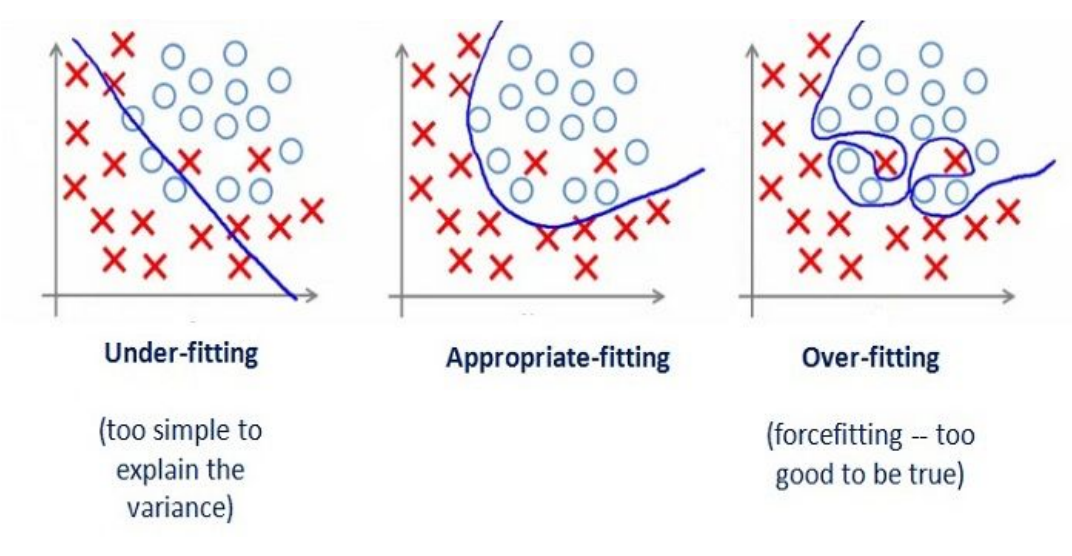
\includegraphics[width=0.6\linewidth]{13.1.PNG}
\caption{Недообучение, хороший фит, переобучение.}
\end{figure}

\textbf{Как детектировать это все?}

Вспомним про train и test, будем измерять лосс на них в зависимости от сложности модели (например,
число эпох или норма вектора весов в линейной регрессии).

• Если и на train, и на test лосс падает, то мы уловили не все основополагающие зависимости
$\Longrightarrow$ недообучение.

• Если на train лосс падает, а на test лосс растет, то мы уловили шумовые зависимости, чуждые
распределению $\Longrightarrow$ переобучение

Подробнее разберём вопрос: переобучение и недообучение. Когда мы просто запоминаем точки из тренировочной выборки, у нас будет не модель, которая будет возможно проходить через все точки на train, но на реальных данных показывать плохие результаты, модель скорее всего будет слишком сложной. А также если наша модель недообучилась, то будет слишком простая, неподходящая под реальность модель. Чем больше мы увеличиваем сложность моделей, тем больше данных нам нужно, чтобы её пофитить, но тем больше у нас возможностей изучить сложные закономерности. Чтобы баланс не нарушить, то есть иметь оптимальное обучение без недообучения и переобучения, нам нужно соблюдать все 3 этапа жизненного цикла построения модели (следует из bias variance decomposition). Оптимальной сложностью или временем обучения нейросети, является тот момент, когда значение функции потерь на валидационной выборке начинает расти при падении значения функции потерь на тренировочной выборке. Хорошо это понять можно по картинке ниже или при построении подобных графиков в реальной жизни - на следующем рисунке обучения бинарного классификатора. 


\begin{figure}[h]
\centering
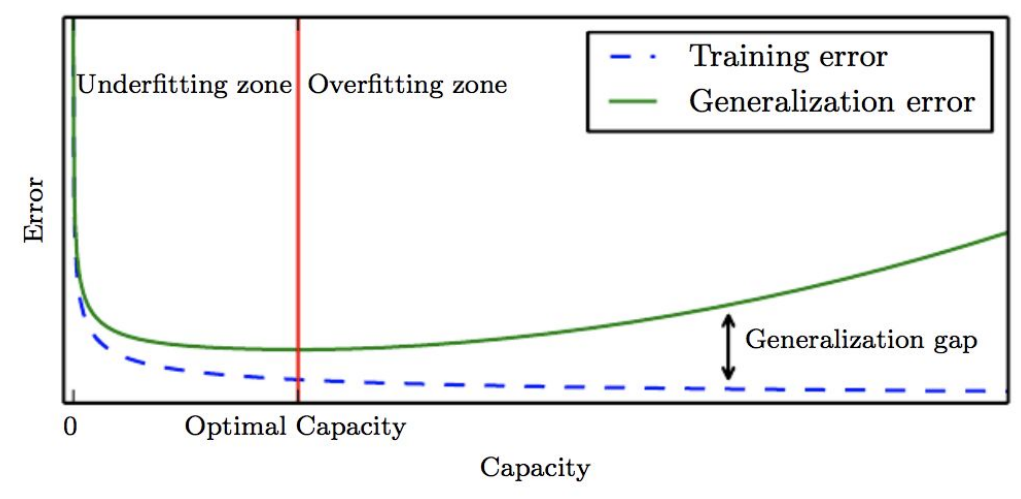
\includegraphics[width=0.5\linewidth]{13.2.PNG}
\caption{Зелёной линией отмечено значение loss function на валидационной выборке, синей линией - на тренировочной. По оси x отмечена сложность модели (эпохи обучения). Красной линией отмечена оптимальная сложность: левее неё недообучение, правее - переобучение.}
\end{figure}

\begin{figure}[h]
\centering
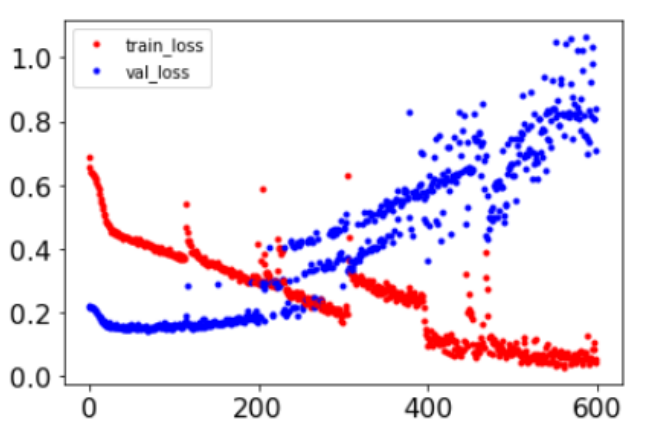
\includegraphics[width=0.4\linewidth]{13.3.PNG}
\caption{Поведение функции потерь бинарного классификатора на валидационной и тренировочной выборке от эпохи обучения нейросети.}
\end{figure}

То есть переобучение - это когда значение функции потерь на валидационной выборке растёт, а на тренировочной падает. Недообучение - когда они все вместе убывают и ещё не надо останавливаться в обучении.

